%PERIMETER \& AREA RELATIONSHIPS - WORKSHEET 0 (IN-CLASS INSTRUCTION)
\documentclass[12pt, letterpaper, fleqn]{article}

% ----------------------------------------------------------
% PACKAGES
% ----------------------------------------------------------
\usepackage{graphicx}
\usepackage{xcolor}
\usepackage[most]{tcolorbox}
\usepackage{amsmath, amssymb}
\usepackage{fancyhdr}
\usepackage[utf8]{inputenc}
\usepackage[T1]{fontenc}
\usepackage{enumitem}
\usepackage{geometry}
\usepackage{tikz}
\usepackage{needspace}
\usepackage{multicol}

\usetikzlibrary{arrows.meta, calc, shapes.geometric}

% ----------------------------------------------------------
% PAGE SETUP
% ----------------------------------------------------------
\usepackage{times}
\geometry{letterpaper, top=1.25in, bottom=1.25in, marginpar=0.5in}

% ----------------------------------------------------------
% HEADER / FOOTER
% ----------------------------------------------------------
\newcommand{\logowidth}{3cm}
\setlength{\headheight}{20pt}
\setlength{\footskip}{40pt}

\pagestyle{fancy}
\fancyhf{}
\fancyhead[C]{\small\bfseries Perimeter \& Area Relationships}
\fancyfoot[L]{\raisebox{2pt}{
\includegraphics[width=\logowidth]{../kss.png}}}
\fancyfoot[C]{\thepage}
\fancyfoot[R]{3.24.0}

\renewcommand{\footrulewidth}{0.2pt}

% ----------------------------------------------------------
% THEME COLOR
% ----------------------------------------------------------
\definecolor{customteal}{HTML}{2fbdb9}

% ----------------------------------------------------------
% HELPER MACROS
% ----------------------------------------------------------
\newcommand{\blank}{\underline{\hspace{2.2cm}}}
\newcommand{\blanklong}{\underline{\hspace{6.5cm}}}
\newcommand{\blankshorter}{\underline{\hspace{1.5cm}}}

% ----------------------------------------------------------
% DOCUMENT
% ----------------------------------------------------------
\begin{document}

\textbf{Name:} \underline{\hspace{5cm}}
\hfill
\textbf{Date:} \underline{\hspace{3cm}}\\

\begin{tcolorbox}[colback=customteal!20]
    \large\textcolor{black}{\textbf{Perimeter of Polygons}}
\end{tcolorbox}

\vspace{3mm}
\noindent
**Perimeter** is the distance all the way **around** the outside of a shape.
To find the perimeter, **add all the side lengths** together.

\begin{tcolorbox}[colback=white, colframe=black!25, boxrule=0.6pt, arc=4mm]
\textbf{Perimeter Example:}
\begin{center}
\begin{tikzpicture}[scale=0.8]
\draw[thick] (0,0) -- (4,0) -- (4,2) -- (0,2) -- cycle;
\node[below] at (2,0) {4 cm};
\node[above] at (2,2) {4 cm};
\node[left] at (0,1) {2 cm};
\node[right] at (4,1) {2 cm};
\end{tikzpicture}
\end{center}
\[
\text{Perimeter} = 4 + 2 + 4 + 2 = 12\text{ cm}
\]
\[
\text{Area} = 4 \times 2 = 8\text{ square cm}
\]
\end{tcolorbox}

\newpage
\begin{tcolorbox}[colback=customteal!20]
    \large\textcolor{black}{\textbf{Guided Practice}}
\end{tcolorbox}

\vspace{5mm}
\begin{enumerate}[itemsep=3cm, leftmargin=0.6cm]
\item Find the perimeter of a triangle with side lengths: 5 inches, 5 inches, and 7 inches.
\\
Equation: \blank $+$ \blank $+$ \blank $=$ \blank inches

\item A rectangle has a perimeter of 20 cm. If the length is 6 cm, what is the width?
\\
Calculation: \vspace{2cm}
\\
Width: \blank cm
\end{enumerate}

\end{document}
